

\subsection{Parallel Simulation}

% The good
\subsubsection{Queue}
\paragraph*{Allocation}
The Queue model is one single chain of models. Each kernel gets one connected part of this chain. The result is that the kernels themselves also form a chain where events only travel in one direction.

\paragraph*{Strong and Weak Scaling}
Figure~\ref{fig:Queue_plot_strong} shows the speedup compared to dxex sequential for a fixed problem size. As the amount of kernels increases, the optimistic kernel quickly becomes the worst choice. The difference between dxex conservative and adevs becoming smaller. The same effect can be seen for weak scaling in Figure~\ref{fig:Queue_plot_weak}.\\
In Figure \ref{fig:Queue_allocation} the allocation of the Queue model is visualized. This trace allows us to demonstrate the benchmark results and explain why optimistic is not ideal for such a chain topology as present in Queue. Kernel 2 is dependent on events from kernels 0 and 1 but by definition of the optimistic synchronization protocol it will simulate ahead without waiting for events it depends on. Any simulation it performs will have to be reverted as soon as events from kernels 0 and 1 arrive. When kernel 2 reverts, kernel 3 will inevitably have to revert as well since most of the events it received from kernel 2 are invalidated and marked as such by antimessages. This leads to severe performance degradation, with an increasing probability of cascading reverts as the number of kernels and models per kernels increases.
The speedup of adevs is always in comparison with the runtime of the corresponding dxex sequential benchmark.
\begin{figure}
	\center
	
	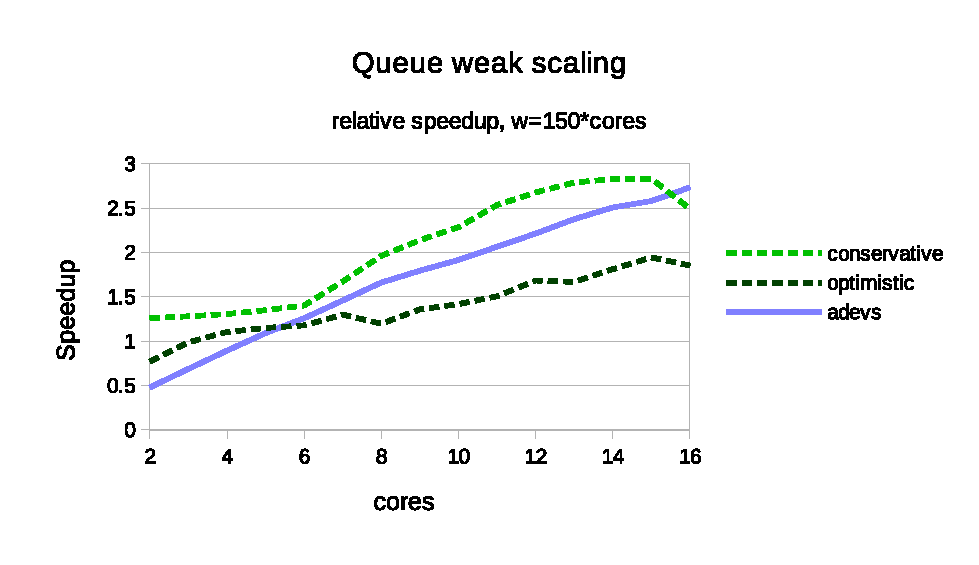
\includegraphics[width=\modelfraction\columnwidth]{fig/queue_fixed_weak_speedup.eps}
	\caption{Queue model weak scaling speedup compared to dxex sequential.}
	\label{fig:Queue_plot_weak}
	
	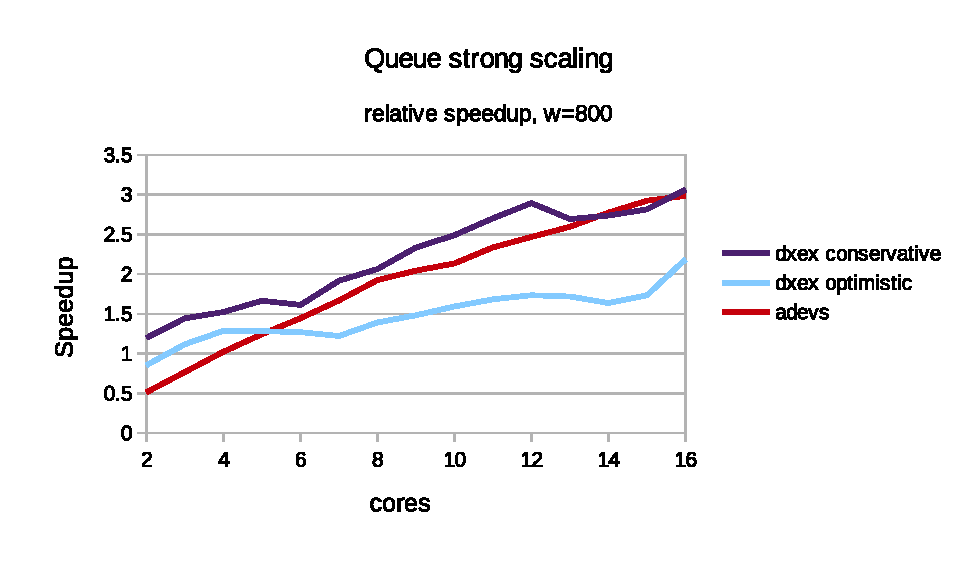
\includegraphics[width=\modelfraction\columnwidth]{fig/queue_fixed_strong_speedup.eps}
	\caption{Queue model strong scaling speedup compared to dxex sequential.}
	\label{fig:Queue_plot_strong}
		
\end{figure}

\begin{figure}
	\center
	
	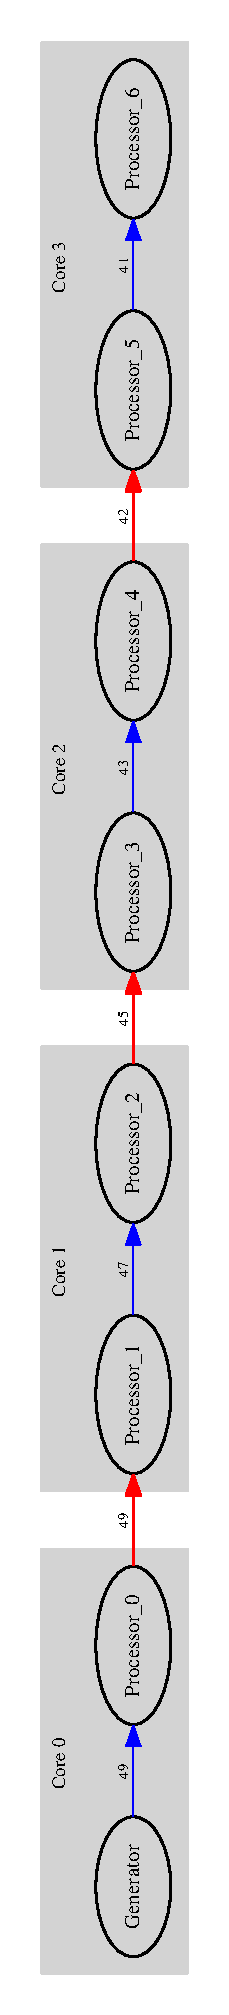
\includegraphics[width=\modelfraction\columnwidth, height=8cm, keepaspectratio, angle=-90 ]{fig/queue_allocation.eps}
	\caption{Queue model (d=2, w=7, t=5000, random timeadvance) allocation and simulation trace across 4 kernels.}
	\label{fig:Queue_allocation}
	
\end{figure}

% The really bad
\subsubsection{Interconnect}\label{subsec:parallelinterconnect}
In the Interconnect model, we determine how broadcast communication is supported across multiple nodes.
The number of models is now kept constant at eight.
Results are shown in Figure~\ref{fig:interconnect_benchmark_parallel}.
When the number of nodes increases, performance decreases due to increasing contention in conservative simulation and an increasing number of of rollbacks in optimistic simulation.
All models depend on each other and have no computational load whatsoever, negating any possible performance gain by executing the simulation in parallel.
In Interconnect there is no allocation scheme possible that avoids cyclic dependencies between simulation kernels, as shown in the trace \ref{fig:interconnect_allocation_parallel} of a simulation with 4 models. Such a cycle forces sequential operation of the kernels with no speedup possible.

\begin{figure}
	\center
	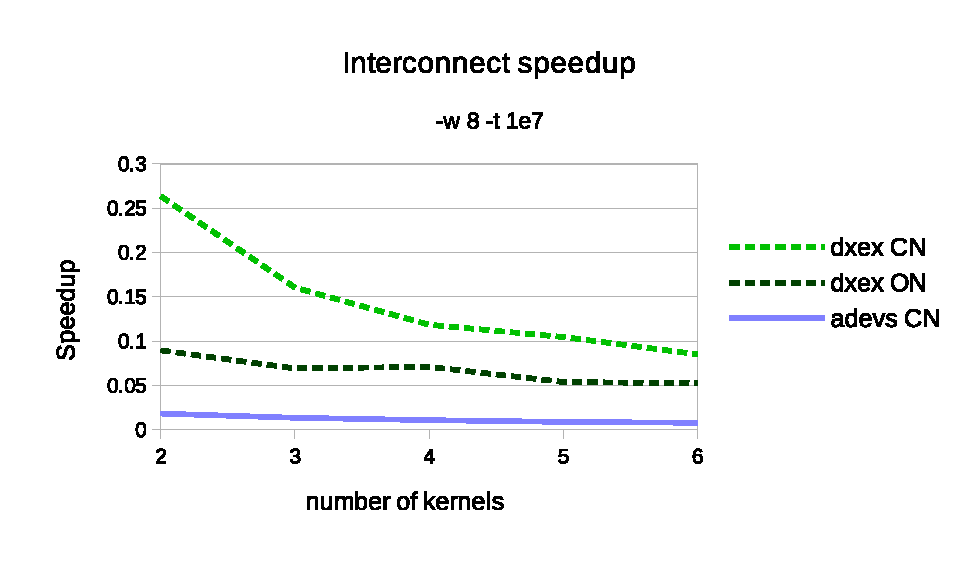
\includegraphics[width=\plotfraction\columnwidth]{fig/interconnect_parallel.eps}
	\caption{Interconnect benchmark results for parallel simulation.}
	\label{fig:interconnect_benchmark_parallel}
\end{figure}
\begin{figure}
	\center
	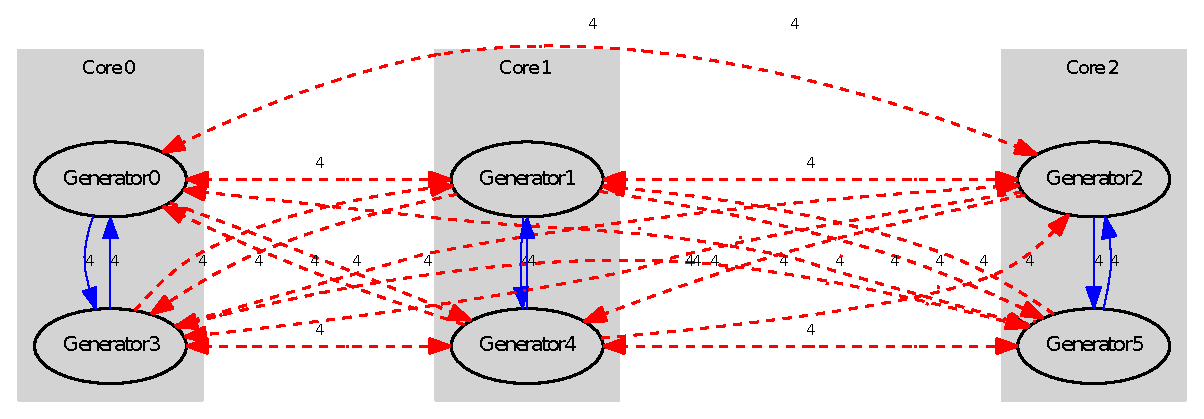
\includegraphics[width=\plotfraction\columnwidth]{fig/interconnect_parallel_allocation.eps}
	\caption{Interconnect parallel simulation trace for 6 models on 3 kernels.}
	\label{fig:interconnect_allocation_parallel}
\end{figure}

% The okayish
\subsubsection{Phold}
% Same cause, different results
In the Phold model, we first investigate the influence of the percentage of remote events on the speedup. A remote event in this context is an event that is sent from a model on one kernel to a model on another simulation kernel.
When remote events are rare, optimistic synchronization rarely has to roll back, thus increasing performance.
With more common remote events, however, optimistic synchronization quickly slows down due to frequent rollbacks.
Conservative synchronization, on the other hand, is mostly unconcerned with the number of remote events: the mere fact that a remote event can happen, causes it to block and wait.
Even though a single synchronization protocol is always ideal in this case, it already shows that different synchronization protocols respond differently to a changing model.
Adevs is significantly slower during conservative synchronization.
Analysis of profiling callgraphs shows that exception handling in adevs is the main cause. 
To keep the models equivalent, the adevs version does not provide the \{begin,end\}Lookahead methods, which accounts for the exception handling. These functions require the user to implement a state saving in contrast to PythonPDEVS and dxex's optimistic kernels which handle this inside the kernel. We feel this would lead to an unfair comparison as we would like to keep the models synchronization-agnostic across all benchmarks.

\begin{figure}
    \center
    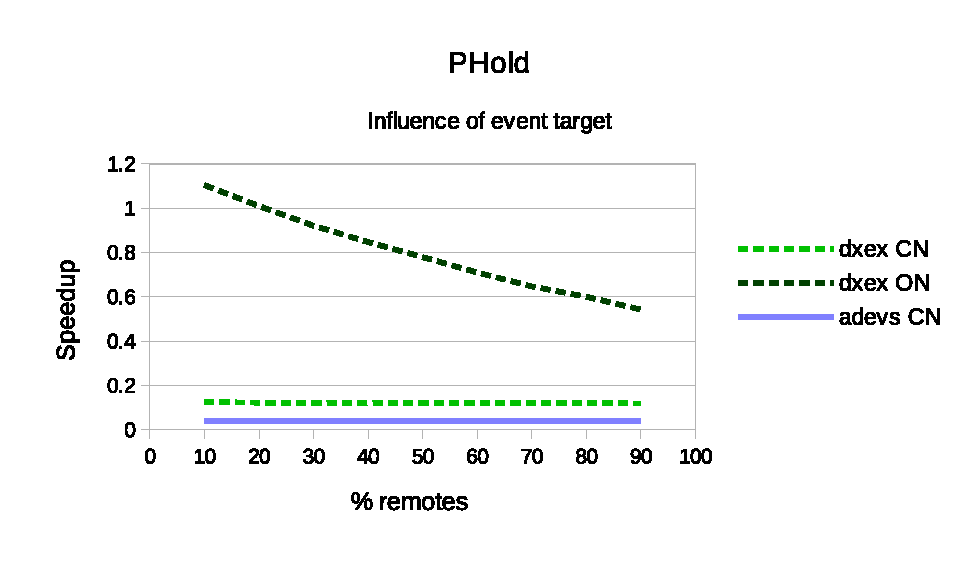
\includegraphics[width=\plotfraction\columnwidth]{fig/phold_remotes.eps}
    \caption{Phold benchmark results for parallel simulation using four kernels, four atomics per node, with varying percentage of remote events.}
\end{figure}
\begin{figure}
	\center
	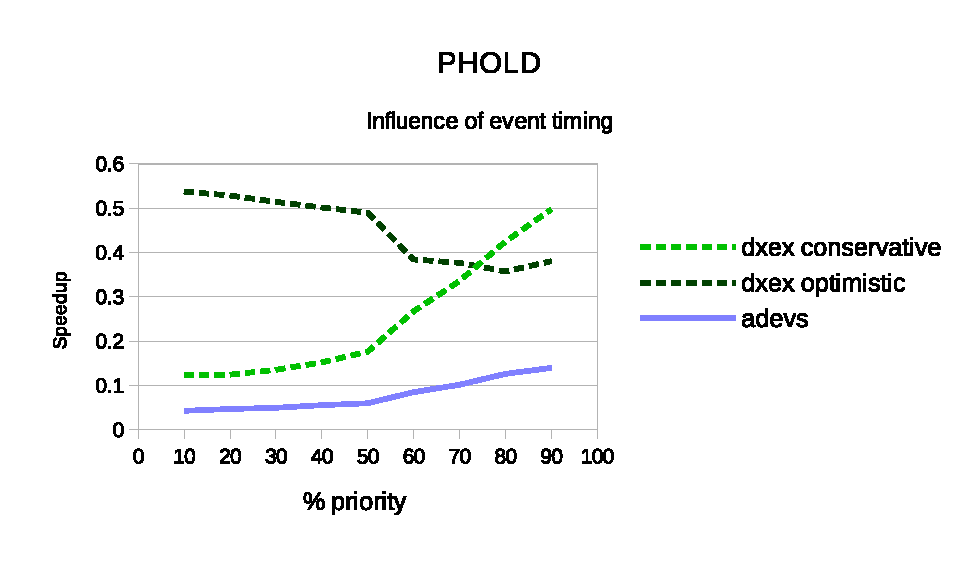
\includegraphics[width=\plotfraction\columnwidth]{fig/phold_priority.eps}
	\caption{Phold benchmark results for parallel simulation using four kernels, with varying amount of high-priority events.}
	\label{fig:phold_priority}
\end{figure}
\begin{figure}
	\center
	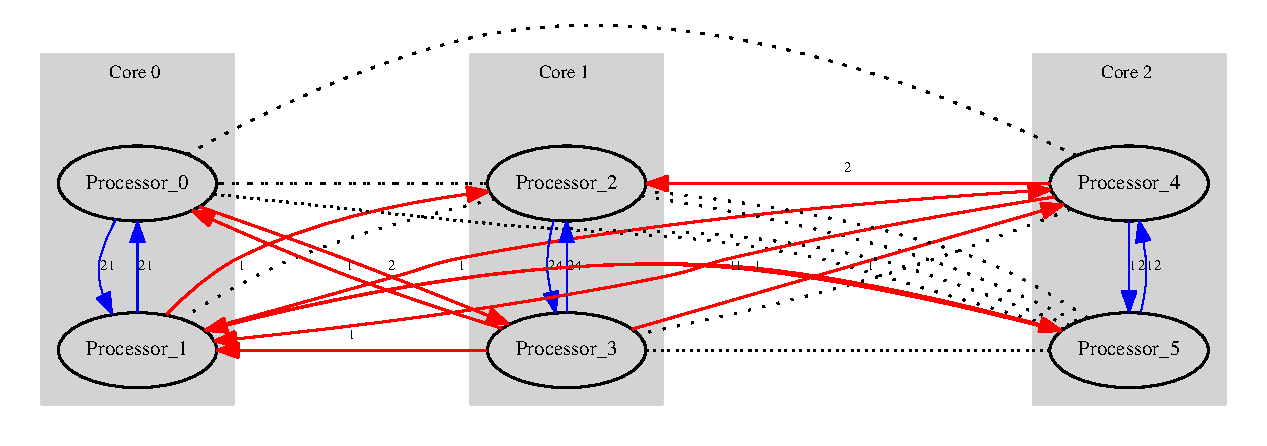
\includegraphics[width=\plotfraction\columnwidth]{fig/phold_parallel_allocation.eps}
	\caption{Phold benchmark trace for parallel simulation using three kernels.}
	\label{fig:phold_allocation}
\end{figure}

We slightly modified the Phold benchmark, to include high-priority events.
Contrary to normal events, high-priority events happen almost instantaneously, restricting lookahead to a very small value.
Even when normal events occur most often, conservative synchronization always blocks until it can make guarantees.
Optimistic synchronization, however, simply goes forward in simulation time and rolls back when these high-priority events happen.
This situation closely mimics the case made in the comparison between both synchronization algorithms by~\cite{FujimotoBook}.
In Figure \ref{fig:phold_allocation} it is clear that in Phold it is possible for dependency cycles to form between kernels which as we have shown in Interconnect degrades performance for both optimistic and conservative. This is also the cause of the sublinear speedup observed in our Phold benchmark.

Figure~\ref{fig:phold_priority} shows how simulation performance is influenced by the fraction of these high-priority events.
If barely any high-priority events occur, conservative synchronization is penalized due to its excessive blocking, which often turned out to be unnecessary.
When many high-priority events occur, optimistic synchronization is penalized due to its mindless progression of simulation, which frequently needs to be rolled back.
Results show that there is no single perfect synchronization algorithm for this model: depending on configuration, either synchronization protocol might be better.


% The real life
\subsubsection{PholdTree}
We further verify that our contribution fulfills our projected use case: a single model that can be tweaked to favor either conservative or optimistic synchronization. We will demonstrate that allocation is critical to achieve a parallel speedup and that the configuration of the model will give either conservative or optimistic an advantage.
\paragraph*{Allocation}\label{PholdTreeallocation}
The PholdTree benchmark can be configured to use 2 allocation schemes: breadth first and depth first. 
The breadth first allocation scheme will result in kernels that will form a dependency chain with multiple branches, much like in the Queue model. 
Such a linear dependency chain can result in a parallel speedup as we demonstrated with the Queue model, but this is not always true as we will demonstrate in this section. 
A single kernel that has an unbalanced number of atomic models or unequal computation load in transition functions will slow down the remainder of the chain. This effect is also apparent if the thread a kernel runs on is not fairly scheduled. In conservative this will lead to excessive polling of the other kernels' eot values, in optimistic this will lead to a cascade of reverts since dependent kernels will simulate ahead of the slower kernel. In Figures \ref{fig:pholdtree_visualize_parBFS} and \ref{fig:pholdtree_visualize_parDFS} the simulation trace is visualized for both allocation schemes highlighting the remarks made in this paragraph.
%
%\begin{figure}
%	\center
%	
%	\includegraphics[width=\modelfraction\columnwidth]{fig/pholdtreeBFS.eps}
%	\caption{PholdTree model breadth first allocation with 3 kernels.}
%	\label{fig:PholdTree_model_bfs}
%	
%	\includegraphics[width=\modelfraction\columnwidth]{fig/pholdtreeDFS.eps}
%	\caption{PholdTree model depth first allocation with 3 kernels.}
%	\label{fig:PholdTree_model_dfs}
%\end{figure}

\paragraph*{Strong Scaling}\label{pholdtreestrongscale}
In Figure \ref{fig:PholdTree_plot_alloc_high} we see that the difference in performance for all 4 kernel configurations compared to that shown in Figure \ref{fig:PholdTree_plot_alloc_low} is a constant factor. The probability of the priority message has no extra impact on performance other than that shown in sequential performance. 

The probability of a high priority event in this model does not affect the performance difference between conservative and optimistic. The key parameter quickly becomes the load of a kernel in models. Our conservative implementation in an uncertain simulation is very sensitive to a high load in models, whereas optimistic has no such limitation.

The difference between depth first and breadth first allocated kernels is striking, the first results in sublinear speedup for both synchronization protocols. %reword 
The breadth first allocation scheme will lead to a very high number of inter-kernel connections, which is detrimental for any parallel synchronization algorithm. An event exchanged between kernels cannot be securely deallocated without a GVT algorithm and all the complexity this entails. Even a fast asynchronous GVT algorithm will require some form of inter kernel synchronization and span a timeframe during which allocated memory cannot be reused, forcing new allocations.
Similar to the Queue benchmark the breadth first allocation scheme leads to a topology for the kernels resembling a chain but with more branches in the chain. In Queue there is only a single model on the edge of a kernel exchanging messages to a single other model in a neighbouring kernel, this is not the case in the PholdTree under breadth first allocation. This explains the difference in speedup between Queue and PholdTree despite the similarity in kernel topology.\\
Depth first allocation still has a higher inter kernel connection count, but not on the same order as breadth first allocated PholdTree. Depth first allocation will converge to a star topology which in this benchmark leads to a significant speedup.\\
The performance drop observed for 2 kernels for all allocation schemes and synchronization protocols is in part due to the higher link count between kernels. With more kernels these connections will be spread across more kernels and result in a relative lower performance penalty. \\
Conservative synchronization suffers a further penalty in this benchmark when there are only a few kernels. The PholdTree model has a lookahead of $\epsilon$ leading the kernel to query each allocated atomic model for a lookahead value on each simulation round. As the atomic models are spread over more kernels this effect is reduced leading to an increase in performance. With 4 kernels conservative surpasses optimistic in speedup. This is clear evidence that conservative synchronization is a good candidate for parallel simulation even in simulations with uncertainty.
\begin{figure}
	\center
	
	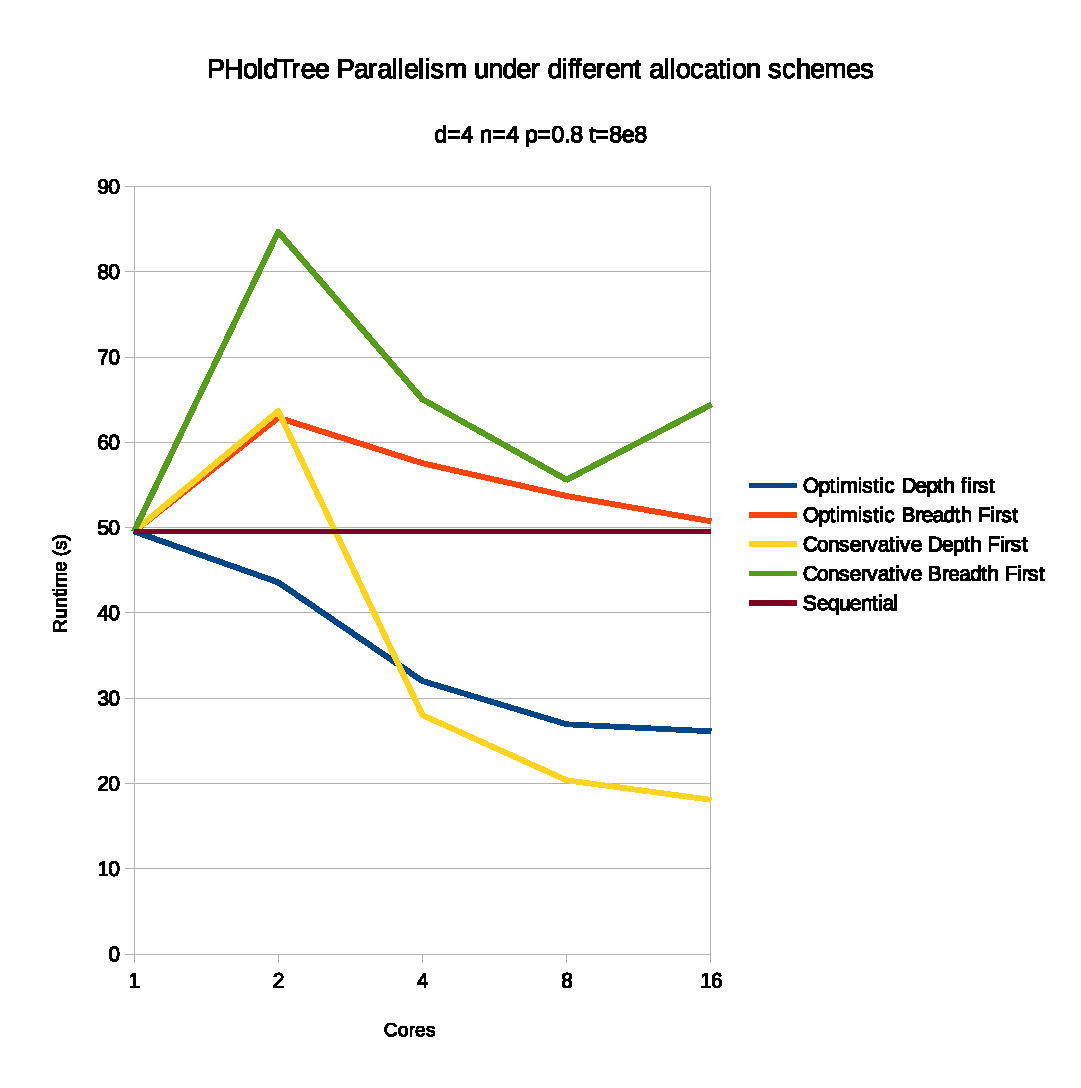
\includegraphics[width=\modelfraction\columnwidth]{fig/pholdtreealloclowp.eps}
	\caption{PholdTree model performance under different allocation schemes with low message probability}
	\label{fig:PholdTree_plot_alloc_low}
	
	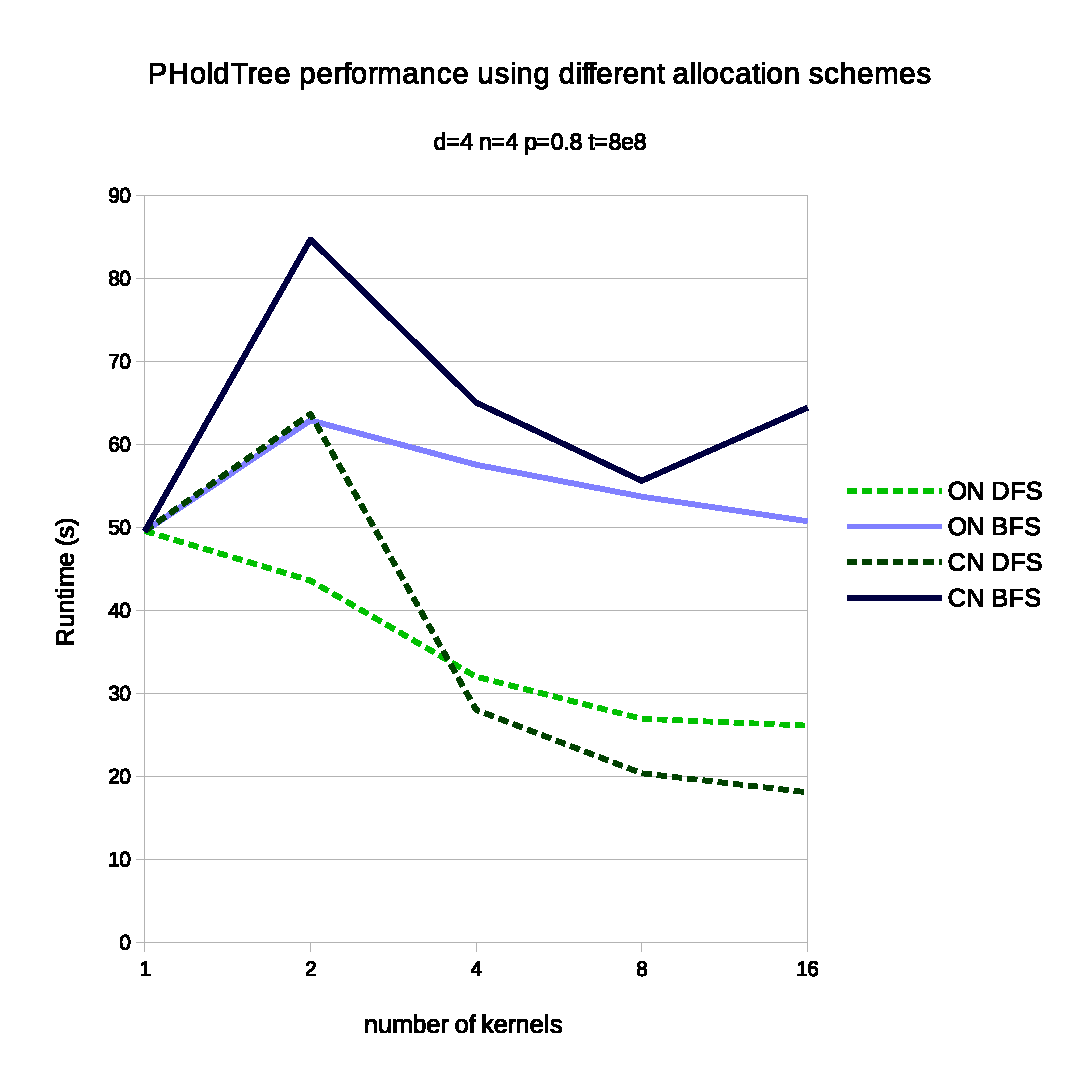
\includegraphics[width=\modelfraction\columnwidth]{fig/pholdtreeallochighp.eps}
	\caption{PholdTree model performance under different allocation schemes with high message probability}
	\label{fig:PholdTree_plot_alloc_high}
\end{figure}

\paragraph*{Weak Scaling}
%Intro
In this paragraph we investigate dxex's parallel performance when the the number of atomic models distributed over a fixed number of kernels varies. From \ref{eq:pholdtreemodelcount} we know that increasing d will lead to a very rapid increase in models. We want to observe what happens in a closer to linear increase in model count per kernel by varying n. 

% Explain why adevs is not plotted (its x100 slower)
Adevs' conservative implementation cannot handle the uncertainty (lack of non $\epsilon$ lookahead) here and is omitted from the comparison. Its parallel performance is two orders of magnitude slower than the sequential implementation. Upon investigation we conclude that this slowdown is caused by not implementing the \{begin/end\}lookahead() functions, which when not overridden in a model trigger an exception on each invocation. 
This exception handling completely stalls the kernel. We do not implement this function in our PholdTree variant for adevs since this would force us to implement state saving in the model code and not use the provided state saving functionality in the kernel, as is done in dxex or PythonPDEVS's optimistic.
In dxex state saving is never required for a conservative simulation, this is handled transparently for the user who need not implement this behaviour. 
By using the state saving technique inside the model code we feel we would no longer compare identical models across different synchronization algorithms, although we do not doubt adevs' increased performance when these functions are overridden.

% Optimistic
In Figure \ref{fig:PholdTree_plot_weaknopt} we observe that dxex's optimistic kernels are slightly sensitive to the number of atomic models allocated to them. In the worst case with 2 kernels there is no real speedup observable, as soon as the number of kernels increases we see a converging speedup trend, that except for 32 kernels is almost constant despite the increase in n. Note that only depth first allocated kernels are measured here, breadth first as we can see in \ref{fig:PholdTree_plot_alloc_high} has no speedup advantage. The probability parameter is kept at 0.1 for the same reason, it only induces a linear increase in load.

% Conservative
Conservative has a more nuanced speedup behaviour in this benchmark. We have detailed how a conservative kernel in dxex scales linear in the number of atomic models (if lookahead is $\epsilon$), this effect is more clearly visible here. \\
It is clear that as the fanout (n) of the model increases the kernel performance degrades rapidly. The intersection of the performance graph of each configuration is shifted to the right, the actual 1-speedup point increases as the kernelcount increases. For a d=4, n=5 configuration with 4 kernels each kernel has a load of ~1300 atomic models when it crosses the 1-speedup line. \\
An 8 kernel configuration with d=4 n=6 can sustain a load of ~2700 atomic models before it reaches that point. From the results we see that the 32-kernel configuration is not yet slowing down with the current parameters. \\
The modelcount is only a part of the explanation of this effect, as the kernelcount increases the amount of inter kernel messages will be split into more distinct sets which can be handled with more concurrency in dxex's architecture. 
That this effect is not always true can be observed from the d=4 n=3 32-kernel datapoint. Note that in this configuration 341 atomic models are distributed over 32 kernels, a relative low model load can more easily highlight synchronization overhead, even if allocation is optimal.\\
As with optimistic we do not include breadth first allocated benchmarks in this speedup plot since none of those achieve a speedup higher than 1.
\\
If we combine both to determine which synchronization protocol is more optimal we see in Figure \ref{fig:PholdTree_plot_weakall} that for these configurations conservative with 8 kernels is an ideal configuration up until n=5, where the modelcount starts to degrade performance. Optimistic with the same kernelcount is almost insensitive to the increase in modelcount and is therefore a more robust choice. Note how optimistic and conservative with 32 kernels at this point still have a reasonable speedup which is surprising given the synchronization overhead in such a large set of kernels.
\begin{figure}
	\center
	
	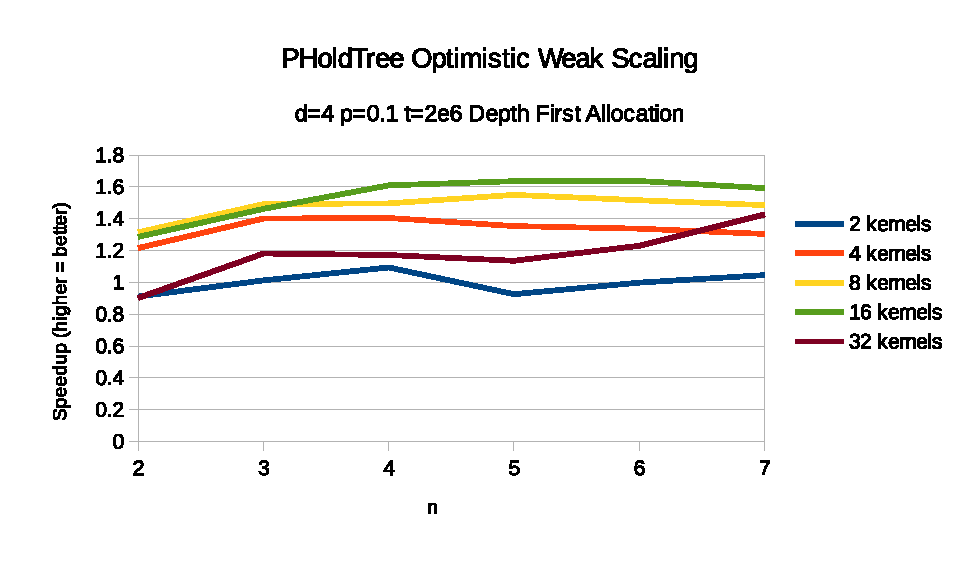
\includegraphics[width=\modelfraction\columnwidth]{fig/pholdtreeweakscalingnopt.eps}
	\caption{PholdTree model weak scaling under varying fanout and optimistic synchronization}
	\label{fig:PholdTree_plot_weaknopt}
	
	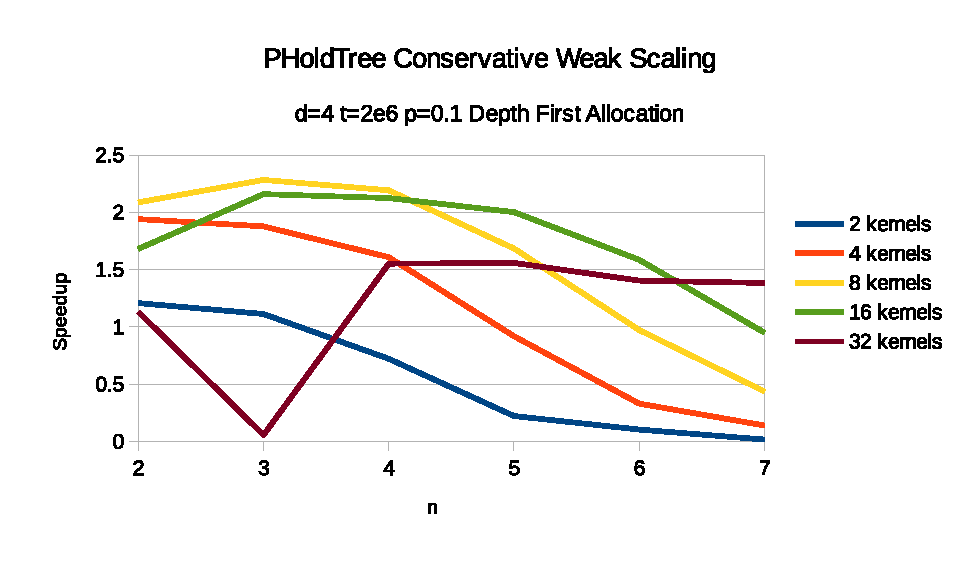
\includegraphics[width=\modelfraction\columnwidth]{fig/pholdtreeweakscalingncon.eps}
	\caption{PholdTree model weak scaling under varying fanout and conservative synchronization}
	\label{fig:PholdTree_plot_weakncon}
	
	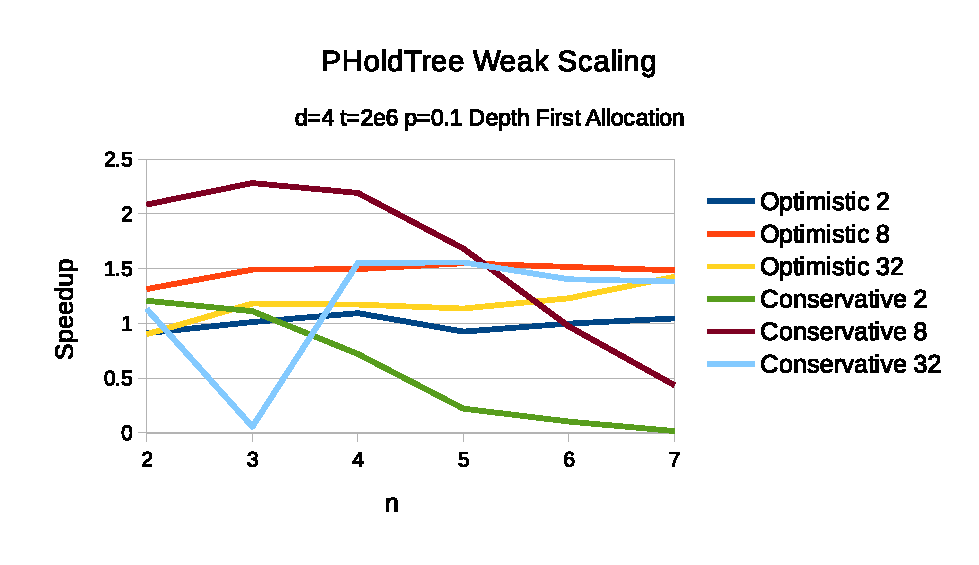
\includegraphics[width=\modelfraction\columnwidth]{fig/pholdtreeweakscalingall.eps}
	\caption{PholdTree model weak scaling under varying fanout and different synchronization algorithms}
	\label{fig:PholdTree_plot_weakall}
		

\end{figure}
